\documentclass[14pt]{extbook}
\usepackage{multicol, enumerate, enumitem, hyperref, color, soul, setspace, parskip, fancyhdr} %General Packages
\usepackage{amssymb, amsthm, amsmath, bbm, latexsym, units, mathtools} %Math Packages
\everymath{\displaystyle} %All math in Display Style
% Packages with additional options
\usepackage[headsep=0.5cm,headheight=12pt, left=1 in,right= 1 in,top= 1 in,bottom= 1 in]{geometry}
\usepackage[usenames,dvipsnames]{xcolor}
\usepackage{dashrule}  % Package to use the command below to create lines between items
\newcommand{\litem}[1]{\item#1\hspace*{-1cm}\rule{\textwidth}{0.4pt}}
\pagestyle{fancy}
\lhead{Progress Quiz 2}
\chead{}
\rhead{Version B}
\lfoot{7862-5421}
\cfoot{}
\rfoot{Spring 2021}
\begin{document}

\begin{enumerate}
\litem{
Solve the equation below. Then, choose the interval that contains the solution.\[ -5(11x + 12) = -14(7x + 13) \]\begin{enumerate}[label=\Alph*.]
\item \( x \in [-5.63, -3.63] \)
\item \( x \in [-2.84, -1.84] \)
\item \( x \in [4.63, 8.63] \)
\item \( x \in [-2.58, -0.58] \)
\item \( \text{There are no real solutions.} \)

\end{enumerate} }
\litem{
Find the equation of the line described below. Write the linear equation as $ y=mx+b $ and choose the intervals that contain $m$ and $b$.\[ \text{Parallel to } 6 x - 5 y = 6 \text{ and passing through the point } (6, 7). \]\begin{enumerate}[label=\Alph*.]
\item \( m \in [0.84, 1.21] \hspace*{3mm} b \in [0.03, 0.3] \)
\item \( m \in [-1.95, -0.77] \hspace*{3mm} b \in [13.57, 14.51] \)
\item \( m \in [0.84, 1.21] \hspace*{3mm} b \in [-0.43, -0.13] \)
\item \( m \in [-0.09, 1.12] \hspace*{3mm} b \in [-0.43, -0.13] \)
\item \( m \in [0.84, 1.21] \hspace*{3mm} b \in [0.84, 1.04] \)

\end{enumerate} }
\litem{
Find the equation of the line described below. Write the linear equation as $ y=mx+b $ and choose the intervals that contain $m$ and $b$.\[ \text{Parallel to } 7 x - 4 y = 14 \text{ and passing through the point } (2, -5). \]\begin{enumerate}[label=\Alph*.]
\item \( m \in [-3.2, -1.1] \hspace*{3mm} b \in [-1.77, -0.45] \)
\item \( m \in [0.3, 1.2] \hspace*{3mm} b \in [-9.89, -8.1] \)
\item \( m \in [0.7, 3.3] \hspace*{3mm} b \in [-9.89, -8.1] \)
\item \( m \in [0.7, 3.3] \hspace*{3mm} b \in [-8, -6.77] \)
\item \( m \in [0.7, 3.3] \hspace*{3mm} b \in [8.43, 9.46] \)

\end{enumerate} }
\litem{
First, find the equation of the line containing the two points below. Then, write the equation as $ y=mx+b $ and choose the intervals that contain $m$ and $b$.\[ (-10, -4) \text{ and } (-11, -3) \]\begin{enumerate}[label=\Alph*.]
\item \( m \in [-3.8, -0.6] \hspace*{3mm} b \in [3, 7] \)
\item \( m \in [-3.8, -0.6] \hspace*{3mm} b \in [8, 12] \)
\item \( m \in [-3.8, -0.6] \hspace*{3mm} b \in [9, 17] \)
\item \( m \in [-3.8, -0.6] \hspace*{3mm} b \in [-15, -7] \)
\item \( m \in [0.2, 3.4] \hspace*{3mm} b \in [8, 12] \)

\end{enumerate} }
\litem{
Solve the linear equation below. Then, choose the interval that contains the solution.\[ \frac{3x -8}{7} - \frac{7x -8}{4} = \frac{-8x -8}{3} \]\begin{enumerate}[label=\Alph*.]
\item \( x \in [-1.7, 0.2] \)
\item \( x \in [-4.4, -1.5] \)
\item \( x \in [-6.3, -5] \)
\item \( x \in [0.1, 2.7] \)
\item \( \text{There are no real solutions.} \)

\end{enumerate} }
\litem{
Write the equation of the line in the graph below in Standard form $Ax+By=C$. Then, choose the intervals that contain $A, B, \text{ and } C$.
\begin{center}
    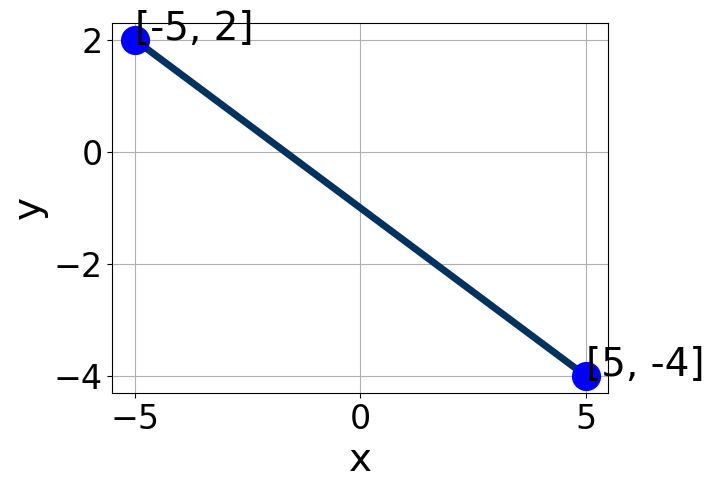
\includegraphics[width=0.5\textwidth]{../Figures/linearGraphToStandardCopyB.png}
\end{center}
\begin{enumerate}[label=\Alph*.]
\item \( A \in [1.4, 7.1], \hspace{3mm} B \in [-5.2, -3.3], \text{ and } \hspace{3mm} C \in [4.2, 6] \)
\item \( A \in [1.4, 7.1], \hspace{3mm} B \in [2.6, 6.7], \text{ and } \hspace{3mm} C \in [-5.6, -4.7] \)
\item \( A \in [-1.1, 1.7], \hspace{3mm} B \in [-2, -0.1], \text{ and } \hspace{3mm} C \in [0.2, 1.2] \)
\item \( A \in [-6.7, -2.3], \hspace{3mm} B \in [-5.2, -3.3], \text{ and } \hspace{3mm} C \in [4.2, 6] \)
\item \( A \in [-1.1, 1.7], \hspace{3mm} B \in [0.3, 2.6], \text{ and } \hspace{3mm} C \in [-1.6, -0.4] \)

\end{enumerate} }
\litem{
Solve the equation below. Then, choose the interval that contains the solution.\[ -2(-7x -10) = -5(19x + 9) \]\begin{enumerate}[label=\Alph*.]
\item \( x \in [-0.27, -0.15] \)
\item \( x \in [-0.44, -0.29] \)
\item \( x \in [-0.61, -0.47] \)
\item \( x \in [0.18, 0.23] \)
\item \( \text{There are no real solutions.} \)

\end{enumerate} }
\litem{
Solve the linear equation below. Then, choose the interval that contains the solution.\[ \frac{3x + 6}{7} - \frac{-4x + 7}{2} = \frac{5x + 9}{4} \]\begin{enumerate}[label=\Alph*.]
\item \( x \in [4.15, 8.15] \)
\item \( x \in [0.45, 3.45] \)
\item \( x \in [-3.79, 0.21] \)
\item \( x \in [5.48, 9.48] \)
\item \( \text{There are no real solutions.} \)

\end{enumerate} }
\litem{
Write the equation of the line in the graph below in Standard form $Ax+By=C$. Then, choose the intervals that contain $A, B, \text{ and } C$.
\begin{center}
    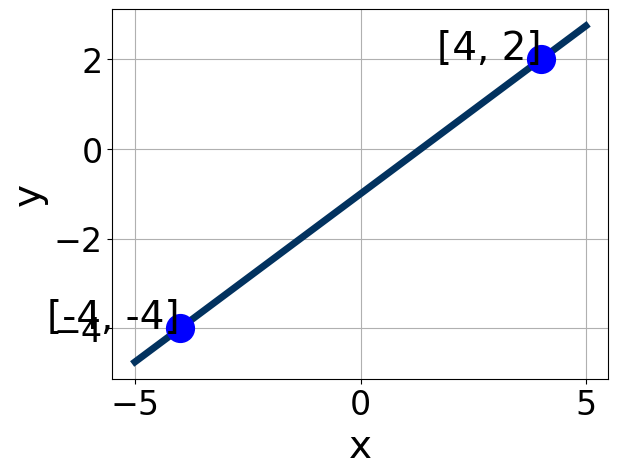
\includegraphics[width=0.5\textwidth]{../Figures/linearGraphToStandardB.png}
\end{center}
\begin{enumerate}[label=\Alph*.]
\item \( A \in [0, 5], \hspace{3mm} B \in [-4.4, -2], \text{ and } \hspace{3mm} C \in [2.6, 6.2] \)
\item \( A \in [-1.75, 2.25], \hspace{3mm} B \in [-0.3, 2.7], \text{ and } \hspace{3mm} C \in [-1.7, 0.3] \)
\item \( A \in [0, 5], \hspace{3mm} B \in [2.1, 4.8], \text{ and } \hspace{3mm} C \in [-6, -3] \)
\item \( A \in [-8, -2], \hspace{3mm} B \in [2.1, 4.8], \text{ and } \hspace{3mm} C \in [-6, -3] \)
\item \( A \in [-1.75, 2.25], \hspace{3mm} B \in [-3.8, 0.8], \text{ and } \hspace{3mm} C \in [0.7, 2.8] \)

\end{enumerate} }
\litem{
First, find the equation of the line containing the two points below. Then, write the equation as $ y=mx+b $ and choose the intervals that contain $m$ and $b$.\[ (-7, 7) \text{ and } (7, 10) \]\begin{enumerate}[label=\Alph*.]
\item \( m \in [0.15, 0.29] \hspace*{3mm} b \in [13.73, 15.34] \)
\item \( m \in [-0.26, -0.16] \hspace*{3mm} b \in [11.06, 11.68] \)
\item \( m \in [0.15, 0.29] \hspace*{3mm} b \in [2.31, 3.35] \)
\item \( m \in [0.15, 0.29] \hspace*{3mm} b \in [-9.69, -6.12] \)
\item \( m \in [0.15, 0.29] \hspace*{3mm} b \in [8.49, 10.11] \)

\end{enumerate} }
\end{enumerate}

\end{document}